%*******************************************************
% Abstract+Sommario
%*******************************************************

\pdfbookmark{Abstract}{Abstract}
\begingroup
\let\clearpage\relax
\let\cleardoublepage\relax
\let\cleardoublepage\relax

\chapter*{Synopsis}
Dorel Industries was established in 1962, and consists of 3 major divisions (Juvenile, Home Furnishings, and Recreational/Leisure).  It owns a wide array of strong brands, including Cosco, Schwinn, Ironhorse, and Mongoose.  While Dorel is a strong player in the bicycle industry, it recently announced (In January of this year) that it would be shuttering its bicycle assembly facilities in the United States and moving to Asia in order to become more competitive.  Annual sales are roughly \$2.6 billion, and with a restructuring of the Recreational/Leisure unit, Dorel expects to save at least \$6 million annually.  Dorel’s primary competitors include Kid Brands, Inc., Trek Bicycle Corporation, and Evenflo Company, Inc.Employs 6,300 people in facilities located in twenty-four countries worldwide.


\vfill
{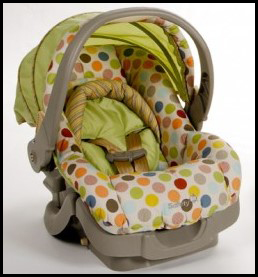
\includegraphics[width=.45\columnwidth]{baby}} 
{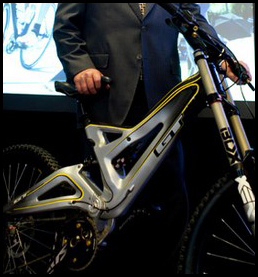
\includegraphics[width=.45\columnwidth]{bike}} 
\vfill
\selectlanguage{italian}
\pdfbookmark[1]{Sommario}{Sommario}
\chapter*{Sommario}
Il pacchetto modifica alcuni aspetti tipografici dello stile \classicthesis, di André Miede. Permette di riprodurre la veste grafica della guida \emph{L'arte di scrivere con \LaTeX}~\citep{pantieri:art}. Lo spunto per l'originale rielaborazione di \classicthesis{} mi è stato offerto da Daniel Gottschlag. Il pacchetto \`e stato scritto per il Gruppo Utilizzatori Italiani di \TeX{} e \LaTeX{} (\url{http://www.guitex.org/}).

\selectlanguage{american}

\endgroup			

\vfill

